\documentclass{beamer}


\mode<presentation>
{
  \usetheme{CambridgeUS}
	\usecolortheme{beaver}
  % or ...

  \setbeamercovered{transparent}
  % or whatever (possibly just delete it)
}


\usepackage{xeCJK}
\usepackage{ulem}
\usepackage[english]{babel}
\usepackage[utf8]{inputenc}
\usepackage{times}
\usepackage[T1]{fontenc}
\usepackage{hyperref}
\usepackage{pifont}
\usepackage{biblatex}
\usepackage{bibentry}
\usepackage{verbatim}
\bibliography{cite}
\newcommand{\cmark}{\ding{51}}%
\newcommand{\xmark}{\ding{55}}%
\setCJKmainfont{WenQuanYi Micro Hei}
\renewcommand{\raggedright}{\leftskip=0pt \rightskip=0pt plus 0cm}
\raggedright

\let\oldfootnotesize\footnotesize
\renewcommand*{\footnotesize}{\oldfootnotesize\tiny}

\title[Intelligent Software Engineering] 
{Intelligent Software Engineering}
\subtitle{Introduction to Artificial Intelligence}

\author[Zhilei Ren] 
{Zhilei Ren}

\institute[Dalian University of Technology] % (optional, but mostly needed)
{
\\
\includegraphics[width=0.1\textwidth]{../utils/logo.png}\\
Dalian University of Technology
}


\subject{Software Engineering}



\pgfdeclareimage[width=0.08\textwidth]{university-logo}{../utils/logo.png}
\logo{\pgfuseimage{university-logo}}



% Delete this, if you do not want the table of contents to pop up at
% the beginning of each subsection:
\AtBeginSubsection[]
{
  \begin{frame}<beamer>{Outline}
    \tableofcontents[currentsection,currentsubsection]
  \end{frame}
}


% If you wish to uncover everything in a step-wise fashion, uncomment
% the following command: 

%\beamerdefaultoverlayspecification{<+->}

\setbeamertemplate{section in toc}[circle]
\setbeamertemplate{items}[circle]
\setbeamertemplate{caption}[numbered]
\setbeamertemplate{bibliography item}{\insertbiblabel}
\setbeamertemplate{bibliography entry title}{}
\setbeamertemplate{bibliography entry journal}{}

\begin{document}

\begin{frame}
  \titlepage
\end{frame}

%\begin{frame}{Outline}
%  \tableofcontents[currentsection,currentsubsection, 
%    hideothersubsections, 
%    sectionstyle=show,
%]
%\end{frame}

\AtBeginSection[]
{
 \begin{frame}<beamer>
 \frametitle{Outline}
 \tableofcontents[currentsection]
 \end{frame}
}
\begin{frame}[t]{bug or feature?}
\end{frame}

\begin{frame}[t]{Vibe Coding}
    Vibe coding is an artificial intelligence-assisted software development style popularized by Andrej Karpathy in February 2025. The term was listed in the Merriam-Webster Dictionary the following month as a ``slang \& trending'' term. It describes a chatbot-based approach to creating software where the developer describes a project or task to a large language model (LLM), which generates code based on the prompt. The developer evaluates the result and asks the LLM for improvements. Unlike traditional AI-assisted coding or pair programming, the human developer avoids micromanaging the code, accepts AI-suggested completions liberally, and focuses more on iterative experimentation than code correctness or structure\footnote{\url{https://en.wikipedia.org/wiki/Vibe_coding}}.
\end{frame}

\begin{frame}[t]{The Illusion of AI Productivity}
    \centering
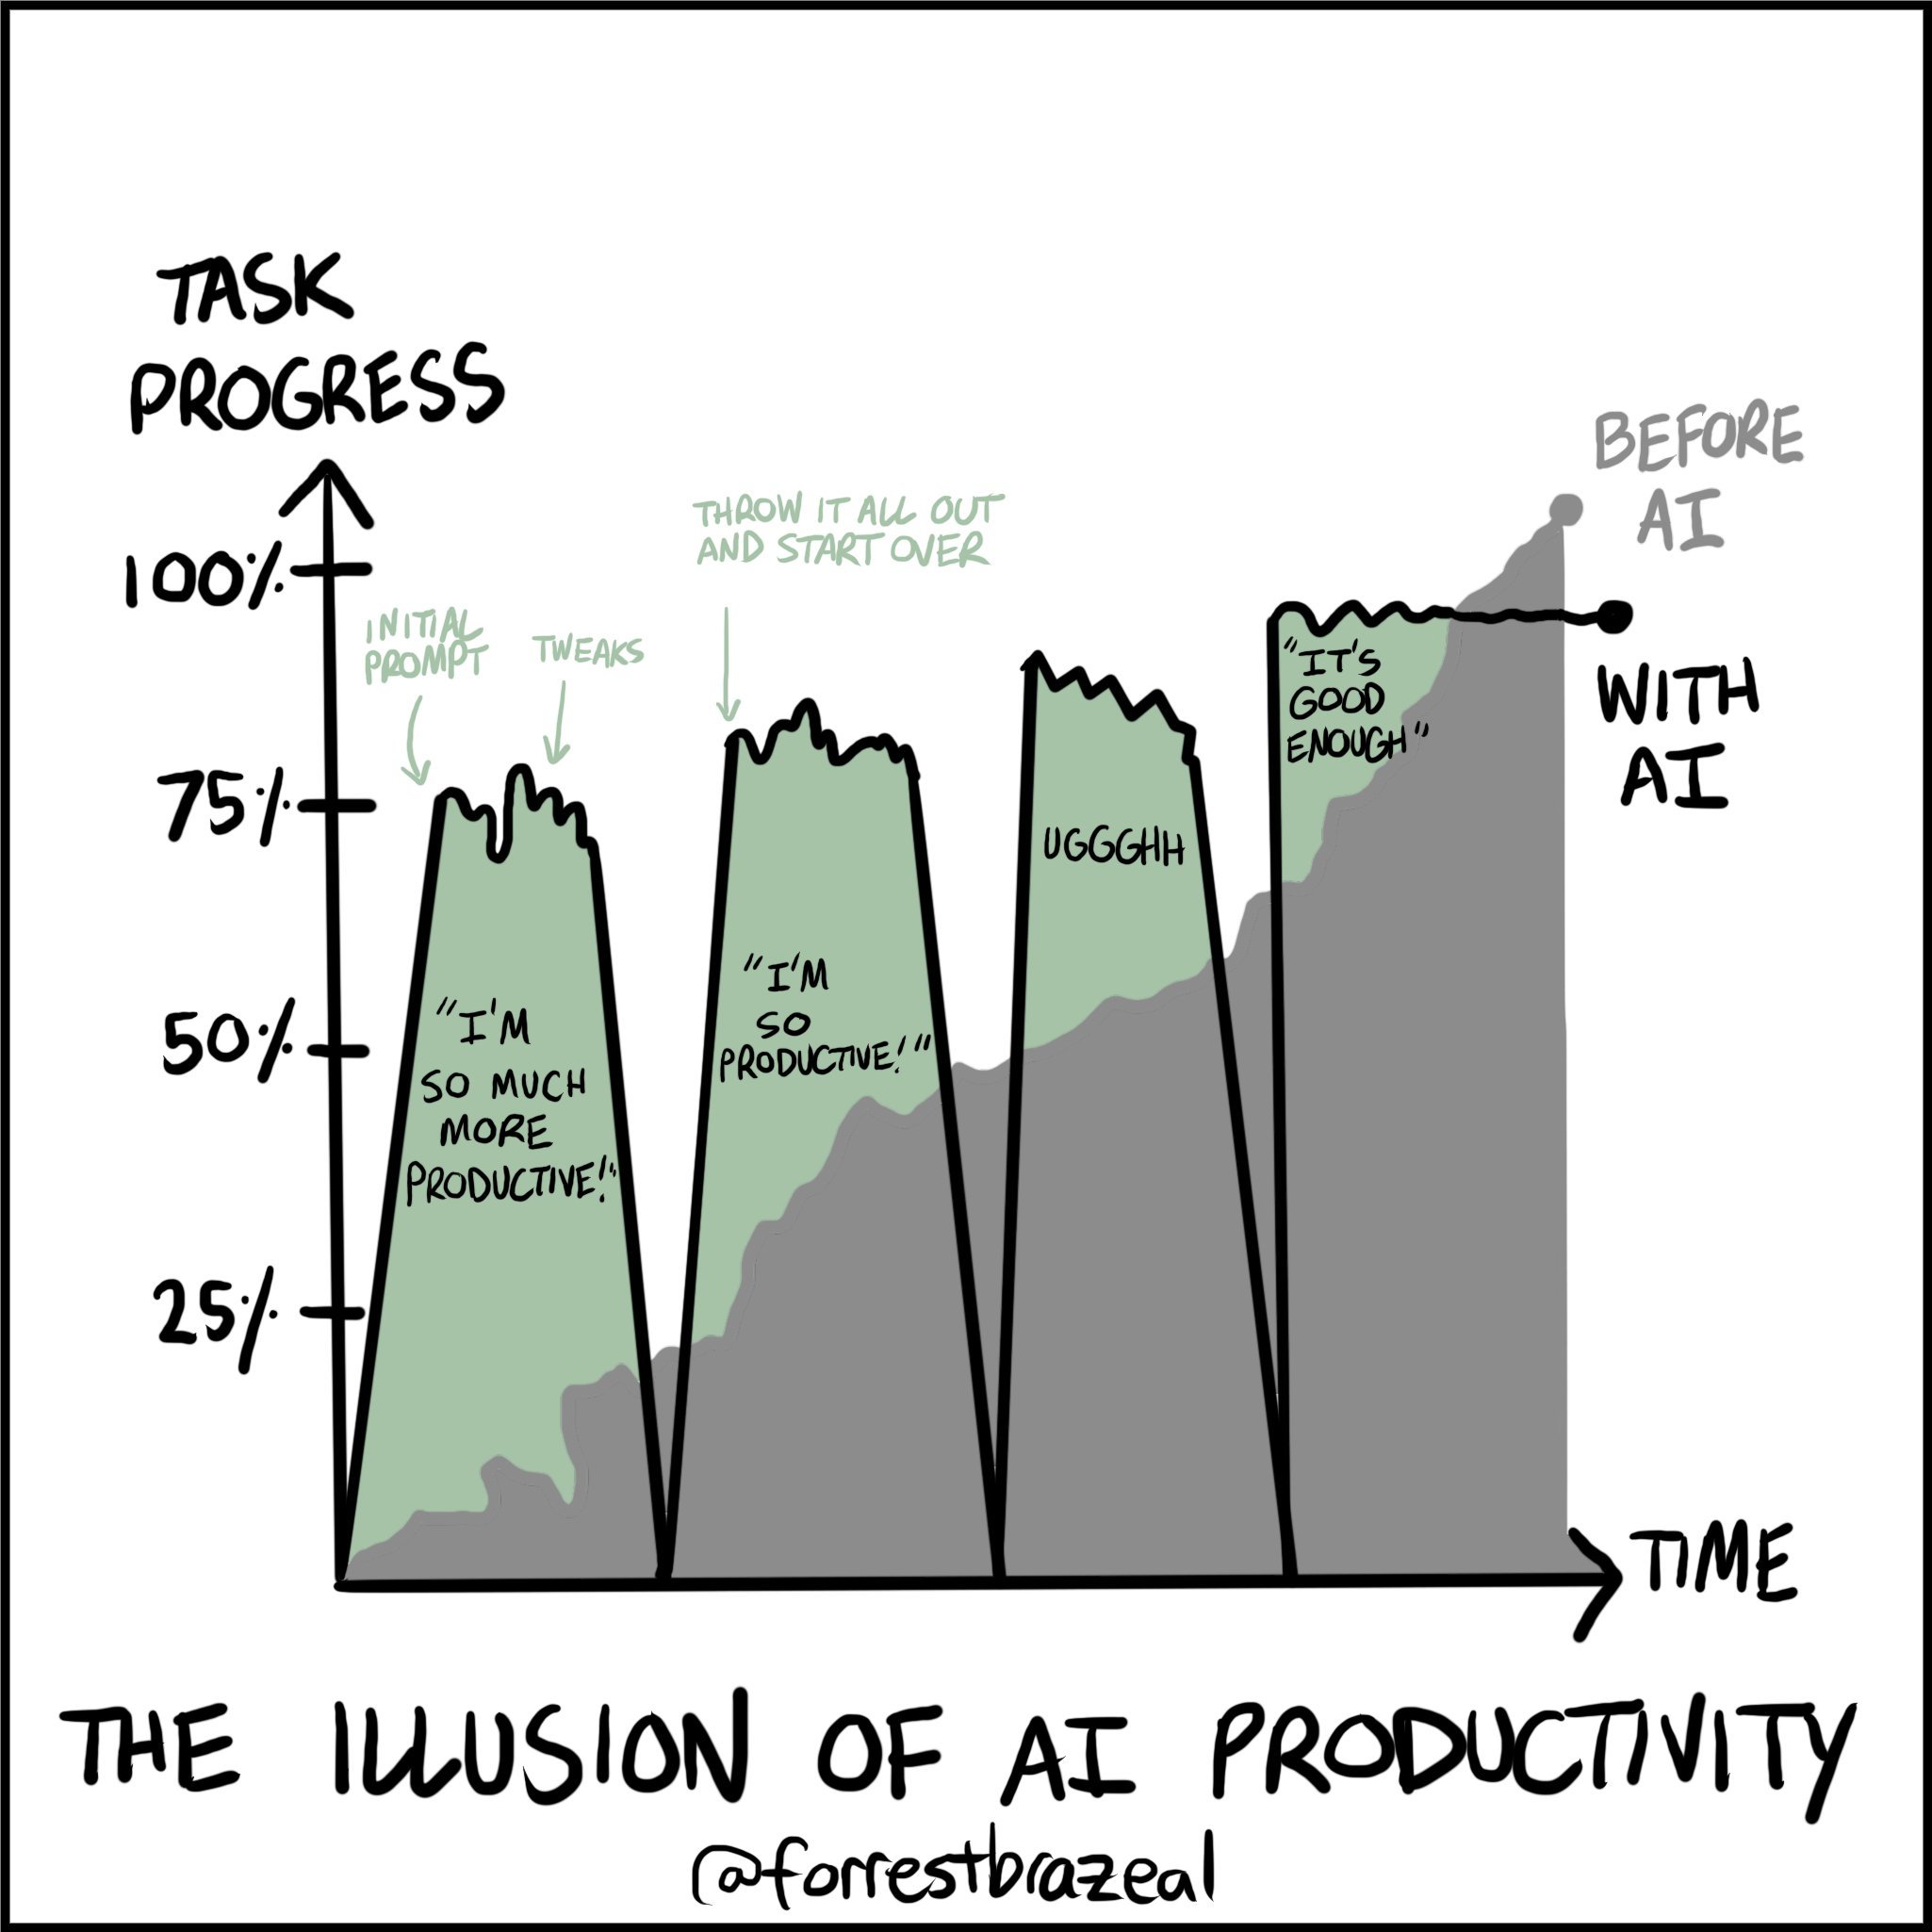
\includegraphics[width=.5\textwidth]{before_ai.jpeg} 
\end{frame}

\begin{frame}[t]{The Mythical Man-Month}

There is no single development, in either technology or management technique, which by itself promises even one order of magnitude [tenfold] improvement within a decade in productivity, in reliability, in simplicity. 
\flushright -- Fred Brooks

\centering


\includegraphics[width=.2\textwidth]{man_month.jpg} 

\end{frame}

\end{document}

